% Options for packages loaded elsewhere
% Options for packages loaded elsewhere
\PassOptionsToPackage{unicode}{hyperref}
\PassOptionsToPackage{hyphens}{url}
%
\documentclass[
  ignorenonframetext,
  aspectratio=169,
]{beamer}
\newif\ifbibliography
\usepackage{pgfpages}
\setbeamertemplate{caption}[numbered]
\setbeamertemplate{caption label separator}{: }
\setbeamercolor{caption name}{fg=normal text.fg}
\beamertemplatenavigationsymbolsempty
% remove section numbering
\setbeamertemplate{part page}{
  \centering
  \begin{beamercolorbox}[sep=16pt,center]{part title}
    \usebeamerfont{part title}\insertpart\par
  \end{beamercolorbox}
}
\setbeamertemplate{section page}{
  \centering
  \begin{beamercolorbox}[sep=12pt,center]{section title}
    \usebeamerfont{section title}\insertsection\par
  \end{beamercolorbox}
}
\setbeamertemplate{subsection page}{
  \centering
  \begin{beamercolorbox}[sep=8pt,center]{subsection title}
    \usebeamerfont{subsection title}\insertsubsection\par
  \end{beamercolorbox}
}
% Prevent slide breaks in the middle of a paragraph
\widowpenalties 1 10000
\raggedbottom
\AtBeginPart{
  \frame{\partpage}
}
\AtBeginSection{
  \ifbibliography
  \else
    \frame{\sectionpage}
  \fi
}
\AtBeginSubsection{
  \frame{\subsectionpage}
}
\usepackage{iftex}
\ifPDFTeX
  \usepackage[T1]{fontenc}
  \usepackage[utf8]{inputenc}
  \usepackage{textcomp} % provide euro and other symbols
\else % if luatex or xetex
  \usepackage{unicode-math} % this also loads fontspec
  \defaultfontfeatures{Scale=MatchLowercase}
  \defaultfontfeatures[\rmfamily]{Ligatures=TeX,Scale=1}
\fi
\usepackage{lmodern}

\usetheme[]{Boadilla}
\usecolortheme[]{default}
\usefonttheme[]{professionalfonts}
\ifPDFTeX\else
  % xetex/luatex font selection
\fi
% Use upquote if available, for straight quotes in verbatim environments
\IfFileExists{upquote.sty}{\usepackage{upquote}}{}
\IfFileExists{microtype.sty}{% use microtype if available
  \usepackage[]{microtype}
  \UseMicrotypeSet[protrusion]{basicmath} % disable protrusion for tt fonts
}{}
\makeatletter
\@ifundefined{KOMAClassName}{% if non-KOMA class
  \IfFileExists{parskip.sty}{%
    \usepackage{parskip}
  }{% else
    \setlength{\parindent}{0pt}
    \setlength{\parskip}{6pt plus 2pt minus 1pt}}
}{% if KOMA class
  \KOMAoptions{parskip=half}}
\makeatother


\usepackage{longtable,booktabs,array}
\newcounter{none} % for unnumbered tables
\usepackage{calc} % for calculating minipage widths
\usepackage{caption}
% Make caption package work with longtable
\makeatletter
\def\fnum@table{\tablename~\thetable}
\makeatother
\usepackage{graphicx}
\makeatletter
\newsavebox\pandoc@box
\newcommand*\pandocbounded[1]{% scales image to fit in text height/width
  \sbox\pandoc@box{#1}%
  \Gscale@div\@tempa{\textheight}{\dimexpr\ht\pandoc@box+\dp\pandoc@box\relax}%
  \Gscale@div\@tempb{\linewidth}{\wd\pandoc@box}%
  \ifdim\@tempb\p@<\@tempa\p@\let\@tempa\@tempb\fi% select the smaller of both
  \ifdim\@tempa\p@<\p@\scalebox{\@tempa}{\usebox\pandoc@box}%
  \else\usebox{\pandoc@box}%
  \fi%
}
% Set default figure placement to htbp
\def\fps@figure{htbp}
\makeatother





\setlength{\emergencystretch}{3em} % prevent overfull lines

\providecommand{\tightlist}{%
  \setlength{\itemsep}{0pt}\setlength{\parskip}{0pt}}



 


\makeatletter
\@ifpackageloaded{tcolorbox}{}{\usepackage[skins,breakable]{tcolorbox}}
\@ifpackageloaded{fontawesome5}{}{\usepackage{fontawesome5}}
\definecolor{quarto-callout-color}{HTML}{909090}
\definecolor{quarto-callout-note-color}{HTML}{0758E5}
\definecolor{quarto-callout-important-color}{HTML}{CC1914}
\definecolor{quarto-callout-warning-color}{HTML}{EB9113}
\definecolor{quarto-callout-tip-color}{HTML}{00A047}
\definecolor{quarto-callout-caution-color}{HTML}{FC5300}
\definecolor{quarto-callout-color-frame}{HTML}{acacac}
\definecolor{quarto-callout-note-color-frame}{HTML}{4582ec}
\definecolor{quarto-callout-important-color-frame}{HTML}{d9534f}
\definecolor{quarto-callout-warning-color-frame}{HTML}{f0ad4e}
\definecolor{quarto-callout-tip-color-frame}{HTML}{02b875}
\definecolor{quarto-callout-caution-color-frame}{HTML}{fd7e14}
\makeatother
\makeatletter
\@ifpackageloaded{caption}{}{\usepackage{caption}}
\AtBeginDocument{%
\ifdefined\contentsname
  \renewcommand*\contentsname{Table of contents}
\else
  \newcommand\contentsname{Table of contents}
\fi
\ifdefined\listfigurename
  \renewcommand*\listfigurename{List of Figures}
\else
  \newcommand\listfigurename{List of Figures}
\fi
\ifdefined\listtablename
  \renewcommand*\listtablename{List of Tables}
\else
  \newcommand\listtablename{List of Tables}
\fi
\ifdefined\figurename
  \renewcommand*\figurename{Figure}
\else
  \newcommand\figurename{Figure}
\fi
\ifdefined\tablename
  \renewcommand*\tablename{Table}
\else
  \newcommand\tablename{Table}
\fi
}
\@ifpackageloaded{float}{}{\usepackage{float}}
\floatstyle{ruled}
\@ifundefined{c@chapter}{\newfloat{codelisting}{h}{lop}}{\newfloat{codelisting}{h}{lop}[chapter]}
\floatname{codelisting}{Listing}
\newcommand*\listoflistings{\listof{codelisting}{List of Listings}}
\makeatother
\makeatletter
\makeatother
\makeatletter
\@ifpackageloaded{caption}{}{\usepackage{caption}}
\@ifpackageloaded{subcaption}{}{\usepackage{subcaption}}
\makeatother

\usepackage{bookmark}
\IfFileExists{xurl.sty}{\usepackage{xurl}}{} % add URL line breaks if available
\urlstyle{same}
\hypersetup{
  pdftitle={Lecture 2: Discrete-Time Markov Chains},
  hidelinks,
  pdfcreator={LaTeX via pandoc}}


\title{\texorpdfstring{Lecture 2: Discrete-Time Markov
Chains}{Lecture 2: Discrete-Time Markov Chains}}
\author{}
\date{}

\begin{document}
\frame{\titlepage}


\section{Absorbing States and Closed
Classes}\label{absorbing-states-and-closed-classes}

\begin{frame}{Absorbing states}
\protect\phantomsection\label{absorbing-states}
In a random walk with an absorbing barrier, reaching the barrier means
that the process remains there permanently.

A state \(i\) is called an \textbf{absorbing state} if \(p_{ii}=1\).

Thus, once the process enters state \(i\),
\(\Pr(X_{n+1}=i\mid X_n=i)=1\), so the process cannot leave state \(i\).

For a random walk with absorbing barriers at \(0\) and \(N\),

\[
p_{00}=1
\qquad\text{and}\qquad
p_{NN}=1.
\]

Hence, both \(0\) and \(N\) are absorbing states.
\end{frame}

\begin{frame}{Absorbing random walk}
\protect\phantomsection\label{absorbing-random-walk}
Consider the random walk on \(S={0,1,\ldots,N}\) with absorbing barriers
at \(0\) and \(N\).

For an interior state \(i\),

\[
p_{i,i+1}=p,
\qquad
p_{i,i-1}=q=1-p.
\]

At the boundaries, \(p_{00}=1\) and \(p_{NN}=1\).

Thus, the process moves between neighbouring interior states until it
reaches either \(0\) or \(N\). Once it reaches a boundary, it remains
there forever.

The two boundary states are therefore \textbf{absorbing states}.
\end{frame}

\begin{frame}{Closed classes}
\protect\phantomsection\label{closed-classes}
An absorbing state is a simple example of a \textbf{closed class}.

A non-empty set of states \(C\) is called a \textbf{closed class} if,
once the process enters \(C\), it cannot move to a state outside \(C\).

Equivalently,

\[
p_{ij}=0
\qquad
\text{for all }i\in C,\ j\notin C.
\]

Thus, a closed class is a set of states from which the process cannot
escape.
\end{frame}

\begin{frame}{Absorbing states as closed classes}
\protect\phantomsection\label{absorbing-states-as-closed-classes}
For the absorbing random walk, the sets

\[
C_1=\{0\}
\qquad\text{and}\qquad
C_2=\{N\}
\]

are closed classes.

For example, from state \(0\),

\[
p_{00}=1
\qquad\text{and}\qquad
p_{0j}=0
\quad\text{for }j\ne0.
\]

Therefore, once the process reaches \(0\), it remains in \(C_1={0}\).

Similarly, once the process reaches \(N\), it remains in \(C_2={N}\).

Thus, in this random walk, the two absorbing states form two separate
closed classes.
\end{frame}

\begin{frame}{Why closed classes matter}
\protect\phantomsection\label{why-closed-classes-matter}
Closed classes describe parts of the state space from which the process
cannot escape.

For the absorbing random walk, once the process reaches either boundary,

\[
0
\qquad\text{or}\qquad
N,
\]

its future behaviour is completely determined: it remains at that state
forever.

This leads to two natural questions:

\begin{enumerate}
\tightlist
\item
  \textbf{Which absorbing state will the process reach?}
\item
  \textbf{How long will it take to reach an absorbing state?}
\end{enumerate}

These correspond to the \textbf{absorption probability} and the
\textbf{expected time to absorption}, which we consider next.
\end{frame}

\begin{frame}{Key idea}
\protect\phantomsection\label{key-idea}
An \textbf{absorbing state} is a state that cannot be left:

\[
p_{ii}=1.
\]

A \textbf{closed class} is a set of states that cannot be left once
entered:

\[
p_{ij}=0
\qquad
\text{for }i\in C,\ j\notin C.
\]

Every absorbing state forms a closed class by itself.

For an absorbing random walk, the boundary states \(0\) and \(N\) are
absorbing states and therefore form two closed classes.
\end{frame}

\section{Absorption Probabilities}\label{absorption-probabilities}

\begin{frame}{From where will the process end?}
\protect\phantomsection\label{from-where-will-the-process-end}
Consider a random walk with absorbing barriers at \(0\) and \(N\),
starting at \(X_0=i\), where \(i\in{1,2,\ldots,N-1}\).

The process eventually reaches one of the absorbing states, \(0\) or
\(N\).

Two probabilities are therefore of interest:

\[
u_i=\Pr(X_T=N\mid X_0=i),
\qquad
1-u_i=\Pr(X_T=0\mid X_0=i),
\]

where \(T=\min{n\geq0:X_n=0\text{ or }X_n=N}\) is the time of
absorption.

The quantity \(u_i\) is called the \textbf{absorption probability at
\(N\)} when the process starts from state \(i\).
\end{frame}

\begin{frame}{Fundamental Questions in Random Walks}
\protect\phantomsection\label{fundamental-questions-in-random-walks}
\begin{figure}[H]

{\centering 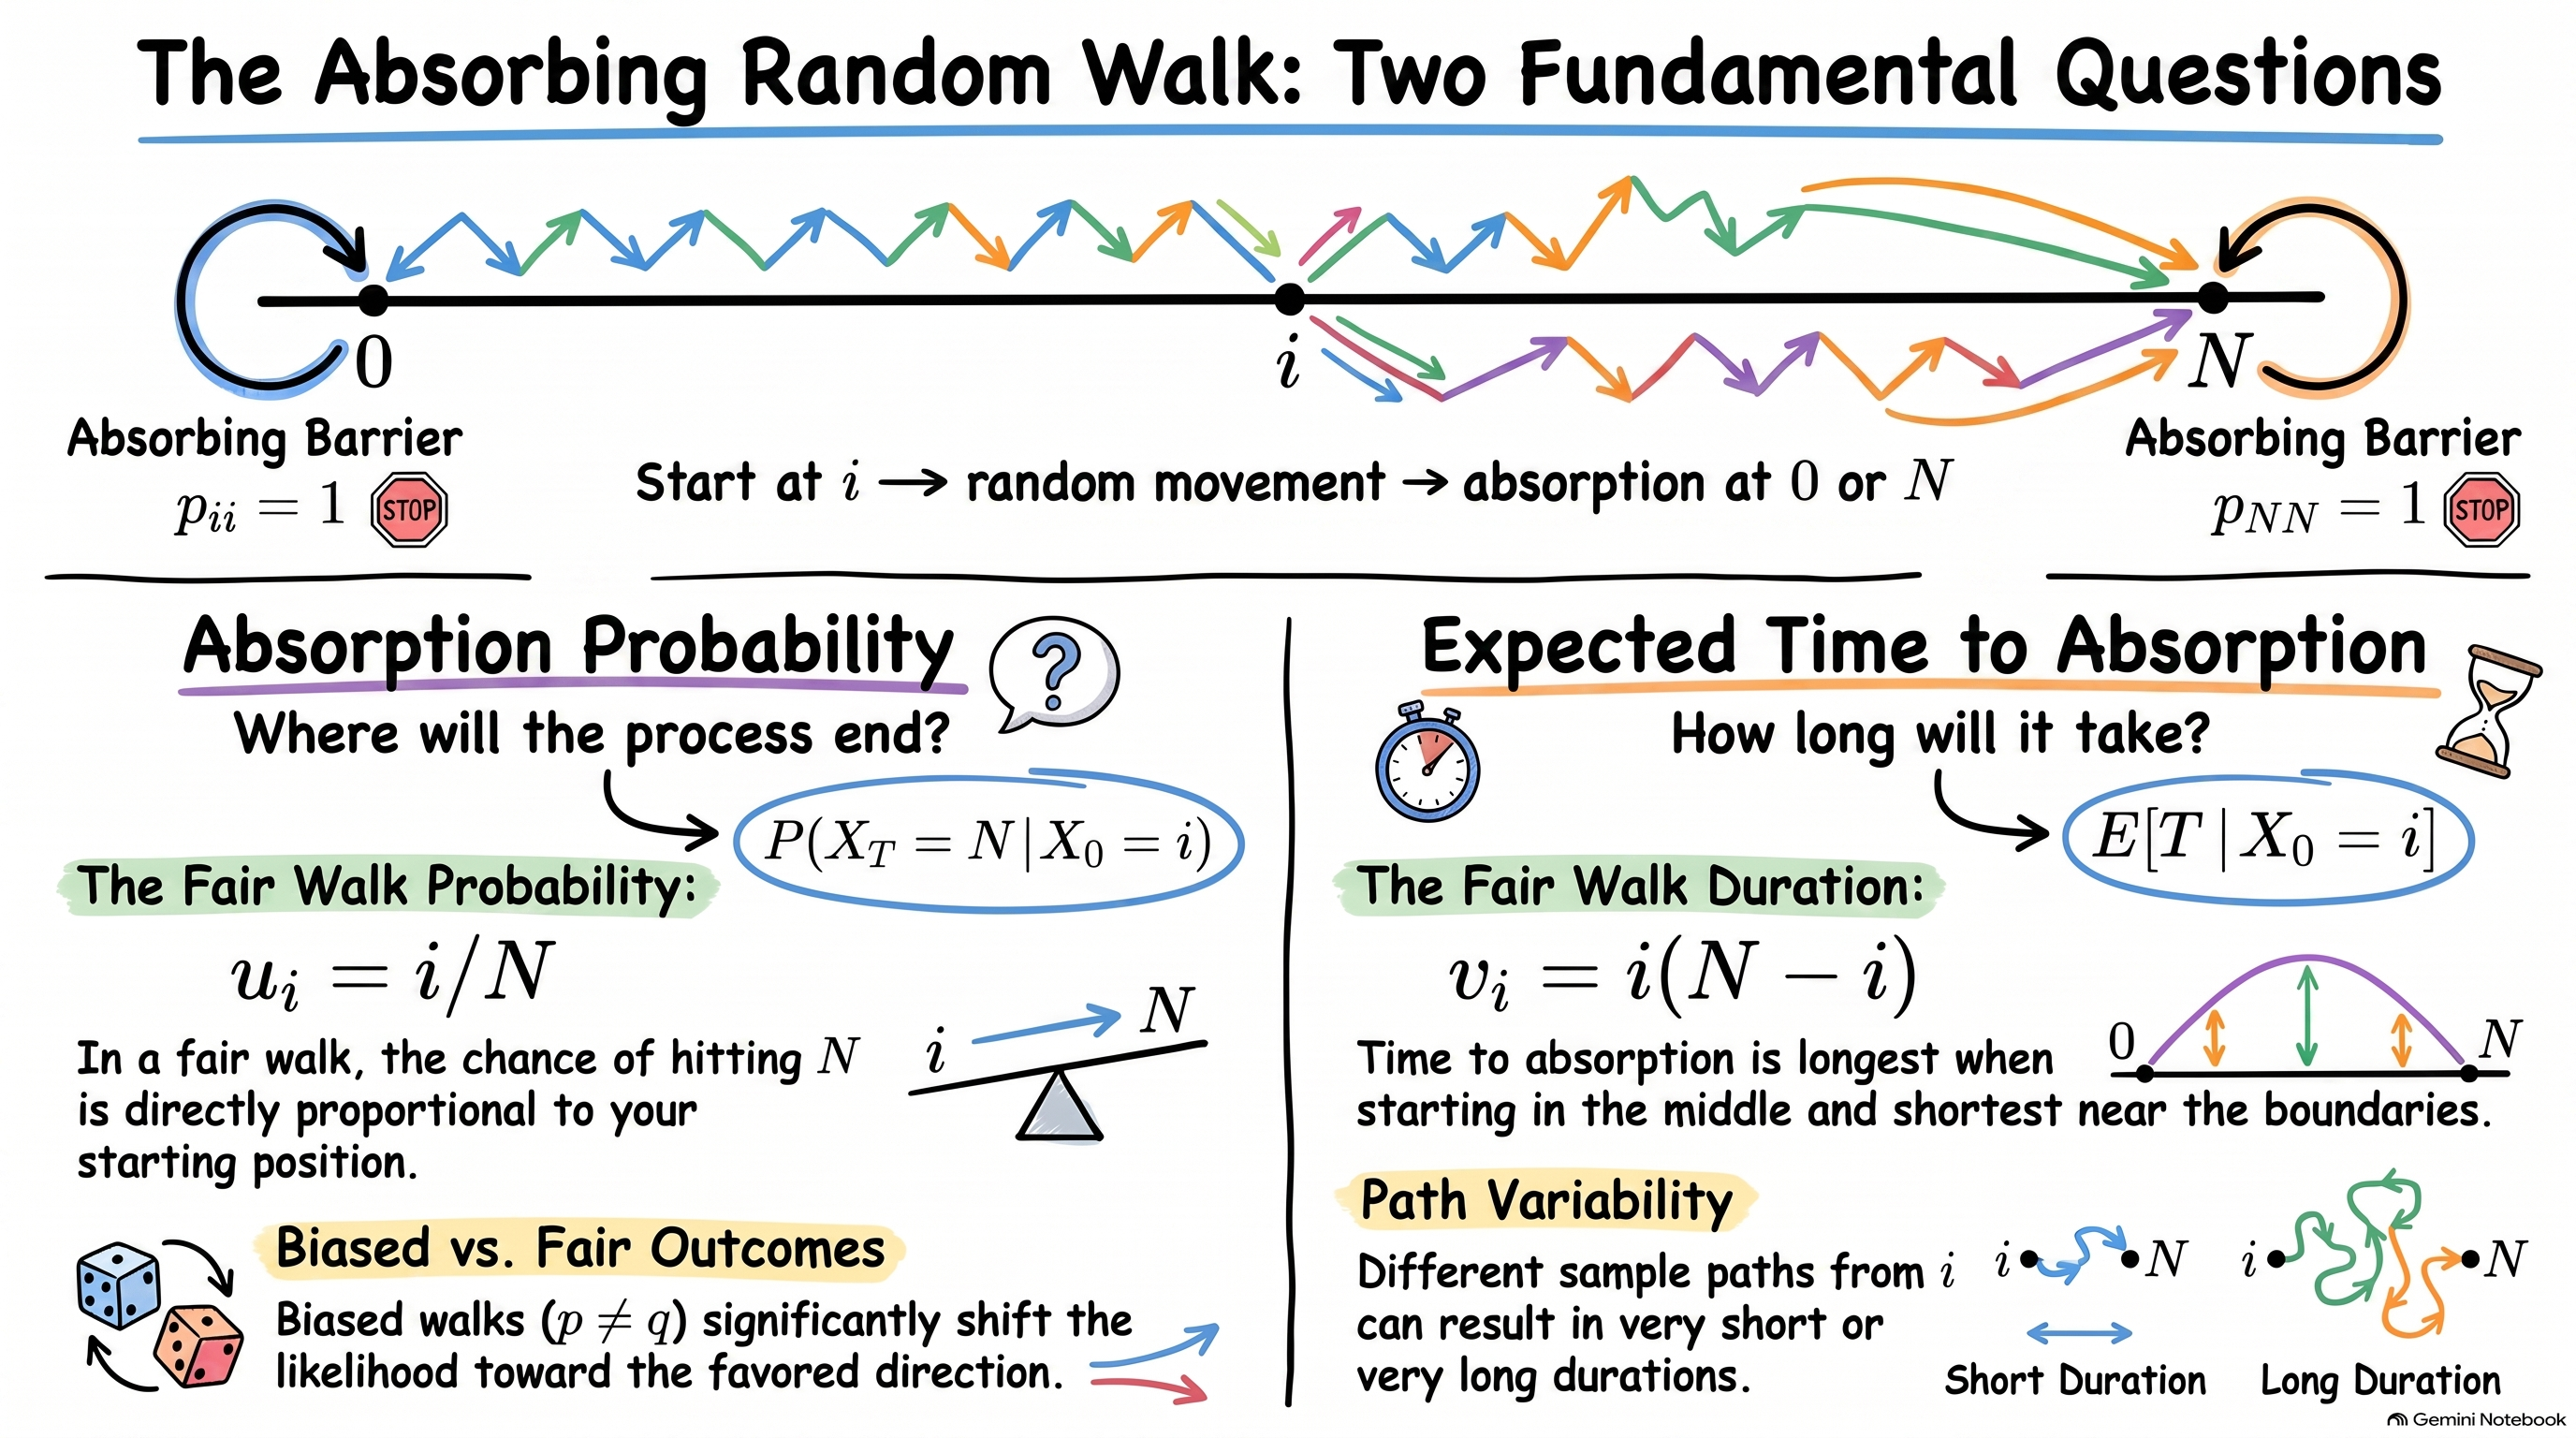
\includegraphics[width=0.7\linewidth,height=\textheight,keepaspectratio]{../figures/Absorbing_Random_Walk_Fundamental_Questions.png}

}

\caption{Fundamental Questions for an Absorbing Random Walk}

\end{figure}%
\end{frame}

\begin{frame}{Boundary conditions}
\protect\phantomsection\label{boundary-conditions}
If the process starts at an absorbing state, the outcome is already
known.

Therefore,

\[
u_0=0
\qquad\text{and}\qquad
u_N=1.
\]

For an interior state \(i\), the value of \(u_i\) depends on the
possible first steps.

If the process starts closer to \(N\), we generally expect \(u_i\) to be
larger.

The absorption probability can therefore be found by considering the
\textbf{first step} of the random walk.
\end{frame}

\begin{frame}{Example: Fair random walk}
\protect\phantomsection\label{example-fair-random-walk}
Consider a fair random walk with absorbing barriers at \(0\) and \(N\).
At each step, the process moves one unit to the right or one unit to the
left with probability \(1/2\). Find the probability that the process is
eventually absorbed at \(N\) when it starts at \(i\), where
\(i\in{1,2,\ldots,N-1}\).

Let

\[
u_i=\Pr(X_T=N\mid X_0=i).
\]

The boundary conditions are \(u_0=0\) and \(u_N=1\).

For an interior state \(i\), the first step gives

\[
u_i=\frac12u_{i+1}+\frac12u_{i-1},
\qquad i=1,2,\ldots,N-1.
\]
\end{frame}

\begin{frame}{Solving the Difference Equation}
\protect\phantomsection\label{solving-the-difference-equation}
Rearranging the first-step equation gives

\[
u_{i+1}-u_i=u_i-u_{i-1}.
\]

Thus, the successive differences are constant, so \(u_i\) is a linear
function of \(i\). Write

\[
u_i=a+bi.
\]

Using \(u_0=0\) and \(u_N=1\),

\[
a=0,
\qquad
a+bN=1.
\]

Hence, \(b=1/N\) and \(\boxed{u_i=\frac{i}{N}}.\)
\end{frame}

\begin{frame}{Absorption probabilities}
\protect\phantomsection\label{absorption-probabilities-1}
Therefore,

\[
\boxed{\Pr(X_T=N\mid X_0=i)=\frac{i}{N}}.
\]

The probability of absorption at \(0\) is

\[
\boxed{
\Pr(X_T=0\mid X_0=i)
=
1-\frac{i}{N}
=
\frac{N-i}{N}
}.
\]
\end{frame}

\begin{frame}{Interpretation}
\protect\phantomsection\label{interpretation}
For a fair random walk, the probability of reaching the upper barrier is
proportional to the starting position.

For example, if \(N=10\) and \(i=4\),

\[
\Pr(X_T=10\mid X_0=4)=\frac4{10}=0.4.
\]

The probability of reaching \(0\) first is

\[
\Pr(X_T=0\mid X_0=4)=\frac6{10}=0.6.
\]

If the process starts halfway between the two barriers, the two
absorbing states are equally likely to be reached first.
\end{frame}

\begin{frame}{Biased random walk}
\protect\phantomsection\label{biased-random-walk}
Now suppose that the random walk moves one step to the right with
probability \(p\) and one step to the left with probability \(q=1-p\).

For an interior state,
\(u_i=pu_{i+1}+qu_{i-1}, \qquad i=1,2,\ldots,N-1,\)

with boundary conditions \(u_0=0 \qquad\text{and}\qquad u_N=1\).

Solving this difference equation gives

\[
\boxed{
u_i=
\begin{cases}
\dfrac{i}{N}, & p=q=\dfrac12,\\[6pt]
\dfrac{1-(q/p)^i}{1-(q/p)^N}, & p\ne q.
\end{cases}}
\]

The fair random walk is therefore a special case of the general result.
\end{frame}

\begin{frame}{Example: Biased Random Walk}
\protect\phantomsection\label{example-biased-random-walk}
Consider a random walk with absorbing barriers at \(0\) and \(10\). At
each step, the process moves one unit to the right with probability
\(p=0.6\) and one unit to the left with probability \(q=0.4\).

If the process starts at \(X_0=4\), find the probability that it is
eventually absorbed at \(10\).

Since \(p\ne q\),

\[
u_i=\frac{1-(q/p)^i}{1-(q/p)^N}.
\]

Here, \(i=4\), \(N=10\), and

\[
\frac{q}{p}=\frac{0.4}{0.6}=\frac{2}{3}.
\]
\end{frame}

\begin{frame}{Example: Biased Random Walk}
\protect\phantomsection\label{example-biased-random-walk-1}
Therefore,

\[
u_4=
\frac{1-(2/3)^4}{1-(2/3)^{10}}
\approx0.817.
\]

Thus,

\[
\boxed{\Pr(X_T=10\mid X_0=4)\approx0.817}.
\]

The probability of absorption at \(0\) is

\[
1-u_4\approx0.183.
\]

The upward bias makes absorption at \(10\) more likely than absorption
at \(0\).
\end{frame}

\section{Expected Time to Absorption}\label{expected-time-to-absorption}

\begin{frame}{How long until absorption?}
\protect\phantomsection\label{how-long-until-absorption}
The absorption probabilities tell us where the random walk is likely to
end. We can also ask how long it takes to reach one of the absorbing
barriers.

For a random walk with absorbing barriers at \(0\) and \(N\), define the
\textbf{time of absorption} by

\[
T=\min\{n\geq0:X_n=0\text{ or }X_n=N\}.
\]

If the process starts at \(X_0=i\), where \(i\in{1,2,\ldots,N-1}\),
define

\[
v_i=\mathrm{E}[T\mid X_0=i].
\]

The value of \(v_i\) depends on the starting position. A process
starting close to an absorbing barrier will generally be absorbed sooner
than one starting near the middle.
\end{frame}

\begin{frame}{Why is the expected time important?}
\protect\phantomsection\label{why-is-the-expected-time-important}
Knowing which outcome is likely to occur is often not enough. We may
also want to know how long it takes for the process to reach that
outcome.

The expected time to absorption provides a measure of the average
duration until an absorbing event occurs.

For example, in an actuarial model, absorption might represent
\textbf{ruin, failure, or termination}. We may therefore want to know
both

\begin{itemize}
\tightlist
\item
  the probability of the absorbing outcome; and
\item
  the expected time until that outcome occurs.
\end{itemize}
\end{frame}

\begin{frame}{Example: Fair random walk}
\protect\phantomsection\label{example-fair-random-walk-1}
Consider a fair random walk with absorbing barriers at \(0\) and \(N\).
At each step, the process moves one unit to the right or one unit to the
left with probability \(1/2\).

Find the expected time to absorption when the process starts at \(i\),
where \(i\in{1,2,\ldots,N-1}\).

Let \(v_i=\mathrm{E}[T\mid X_0=i].\)

Since \(0\) and \(N\) are absorbing,

\[
v_0=0
\qquad\text{and}\qquad
v_N=0.
\]

For an interior state \(i\), the first step takes one unit of time.
After that, the process is at either \(i+1\) or \(i-1\). Therefore,

\[
v_i=1+\frac12v_{i+1}+\frac12v_{i-1}.
\]
\end{frame}

\begin{frame}{Example: Fair random walk}
\protect\phantomsection\label{example-fair-random-walk-2}
Rearranging gives

\[
v_{i+1}-2v_i+v_{i-1}=-2.
\]

The solution to this difference equation is \(v_i=-i^2+ai+b\).

Using \(v_0=0\) and \(v_N=0\) gives

\[
b=0,
\qquad
-N^2+aN=0.
\]

Hence, \(a=N\), so

\[
\boxed{v_i=i(N-i)}.
\]

Thus, for a fair random walk, the expected time to absorption is largest
when the process starts near the middle and decreases as the starting
point approaches either absorbing barrier.
\end{frame}

\begin{frame}{Example: Fair random walk}
\protect\phantomsection\label{example-fair-random-walk-3}
Suppose \(N=10\) and the process starts at \(X_0=4\).

Using

\[
v_i=i(N-i),
\]

we obtain

\[
\mathrm{E}[T\mid X_0=4]
=
4(10-4)
=
24.
\]

Thus, the expected time to absorption is

\[
\boxed{24\text{ steps}}.
\]

For comparison, if the process starts at \(X_0=5\),

\[
\mathrm{E}[T\mid X_0=5]=5(10-5)=25.
\]

The expected time is largest at the middle of the interval.
\end{frame}

\begin{frame}{Example: Biased random walk}
\protect\phantomsection\label{example-biased-random-walk-2}
Suppose the random walk moves one unit to the right with probability
\(p\) and one unit to the left with probability \(q=1-p\).

For an interior state \(i\),

\[
v_i=1+pv_{i+1}+qv_{i-1},
\qquad i=1,2,\ldots,N-1,
\]

with \(v_0=0 \qquad\text{and}\qquad v_N=0.\)

For \(p\ne q\), solving this difference equation gives

\[
\boxed{
v_i=
\frac{
N\dfrac{1-(q/p)^i}{1-(q/p)^N}-i
}{
p-q
}
}.
\]

When \(p=q=1/2\), the result is instead \(\boxed{v_i=i(N-i)}.\)
\end{frame}

\begin{frame}{Example: Biased random walk}
\protect\phantomsection\label{example-biased-random-walk-3}
Consider a random walk with absorbing barriers at \(0\) and \(10\). At
each step, the process moves one unit to the right with probability
\(p=0.6\) and one unit to the left with probability \(q=0.4\).

If the process starts at \(X_0=4\), find the expected time to
absorption.

Since \(p\ne q\),

\[
v_i=
\frac{
N\dfrac{1-(q/p)^i}{1-(q/p)^N}-i
}{
p-q
}.
\]

Here, \(i=4\), \(N=10\), and

\[
\frac{q}{p}=\frac{0.4}{0.6}=\frac23.
\]
\end{frame}

\begin{frame}{Example: Biased random walk}
\protect\phantomsection\label{example-biased-random-walk-4}
Therefore,

\[
v_4=
\frac{
10\dfrac{1-(2/3)^4}{1-(2/3)^{10}}-4
}{
0.2
}
\approx20.8.
\]

Thus,

\[
\boxed{\mathrm{E}[T\mid X_0=4]\approx20.8\text{ steps}}.
\]

For the fair random walk with the same starting point and barriers,

\[
\mathrm{E}[T\mid X_0=4]=24.
\]

The upward bias changes both the likely absorbing state and the expected
time until absorption.
\end{frame}

\section{First-Step Analysis}\label{first-step-analysis}

\begin{frame}{A general method}
\protect\phantomsection\label{a-general-method}
The calculations for absorption probabilities and expected absorption
times use the same basic idea: \textbf{consider what happens after the
first transition}.

Starting from state \(i\), identify all states that can be reached in
one step. The Markov property then allows us to treat the process after
that first step as a new process starting from the state reached.

This produces an equation for the quantity of interest.
\end{frame}

\begin{frame}{Absorption probabilities}
\protect\phantomsection\label{absorption-probabilities-2}
Consider a Markov chain with an absorbing set \(A\). Let
\(u_i=\Pr(\text{the process is eventually absorbed in }A\mid X_0=i)\).

For a state \(i\) outside \(A\), condition on the state reached after
the first transition. By the law of total probability and the Markov
property,

\[
u_i=\sum_{j\in S}p_{ij}u_j.
\]

For an absorbing state in \(A\), \(u_i=1\). For an absorbing state
outside \(A\), \(u_i=0\).

These boundary conditions, together with the first-step equations for
the remaining states, determine the absorption probabilities.
\end{frame}

\begin{frame}{Example: Absorption probability}
\protect\phantomsection\label{example-absorption-probability}
Consider the Markov chain with state space \(S={0,1,2}\) and transition
matrix

\[
P=
\begin{bmatrix}
1&0&0\\
p_{10}&p_{11}&p_{12}\\
0&0&1
\end{bmatrix}.
\]

States \(0\) and \(2\) are absorbing. Find the probability that the
process is eventually absorbed at state \(0\), given that it starts at
state \(1\).

Let \(u_i=\Pr(X_T=0\mid X_0=i)\), where
\(T=\min{n\geq0:X_n=0\text{ or }X_n=2}\).

The boundary conditions are \(u_0=1\) and \(u_2=0\).
\end{frame}

\begin{frame}{Example: Absorption probability}
\protect\phantomsection\label{example-absorption-probability-1}
Starting from state \(1\), the first transition can lead to states
\(0\), \(1\), or \(2\). Therefore,

\[
u_1=p_{10}u_0+p_{11}u_1+p_{12}u_2.
\]

Using \(u_0=1\) and \(u_2=0\), \(u_1=p_{10}+p_{11}u_1\), so

\[
u_1=\frac{p_{10}}{1-p_{11}}.
\]

Since the entries in row \(1\) sum to \(1\), \(1-p_{11}=p_{10}+p_{12}\).
Therefore,

\[
\boxed{u_1=\frac{p_{10}}{p_{10}+p_{12}}}.
\]

The probability of eventual absorption at state \(0\) depends on the
relative probabilities of leaving state \(1\) towards the two absorbing
states.
\end{frame}

\begin{frame}{Expected time to absorption}
\protect\phantomsection\label{expected-time-to-absorption-1}
First-step analysis can also be used to find the expected time until
absorption.

Let \(v_i=\mathrm{E}[T\mid X_0=i]\), where \(T\) is the time of
absorption.

For an absorbing state, \(v_i=0\).

For a non-absorbing state \(i\), one transition occurs before the
remaining process begins. Therefore,

\[
v_i=1+\sum_{j\in S}p_{ij}v_j.
\]

The term \(1\) accounts for the first transition.
\end{frame}

\begin{frame}{Example: Expected time to absorption}
\protect\phantomsection\label{example-expected-time-to-absorption}
Consider the Markov chain with state space \(S={0,1,2}\) and transition
matrix

\[
P=
\begin{bmatrix}
1&0&0\\
p_{10}&p_{11}&p_{12}\\
0&0&1
\end{bmatrix}.
\]

States \(0\) and \(2\) are absorbing. Find the expected time to
absorption when the process starts at state \(1\).

Let \(v_i=\mathrm{E}[T\mid X_0=i]\), where
\(T=\min{n\geq0:X_n=0\text{ or }X_n=2}\).

Since states \(0\) and \(2\) are absorbing, \(v_0=0\) and \(v_2=0\).
\end{frame}

\begin{frame}{Example: Expected time to absorption}
\protect\phantomsection\label{example-expected-time-to-absorption-1}
Starting from state \(1\), one transition occurs first. Hence,

\[
v_1=1+p_{10}v_0+p_{11}v_1+p_{12}v_2.
\]

Using \(v_0=v_2=0\),

\[
v_1=1+p_{11}v_1.
\]

Therefore,

\[
\boxed{v_1=\frac{1}{1-p_{11}}}.
\]

The quantity \(1-p_{11}\) is the probability of leaving state \(1\) on
each step. A larger probability of remaining in state \(1\) therefore
gives a larger expected time to absorption.
\end{frame}

\begin{frame}{A system of first-step equations}
\protect\phantomsection\label{a-system-of-first-step-equations}
When there are several non-absorbing states, first-step analysis
produces a system of simultaneous equations.

Consider a Markov chain with state space \(S={0,1,2,3}\) and transition
matrix

\[
P=
\begin{bmatrix}
1&0&0&0\\
p_{10}&p_{11}&p_{12}&p_{13}\\
p_{20}&p_{21}&p_{22}&p_{23}\\
0&0&0&1
\end{bmatrix}.
\]

States \(0\) and \(3\) are absorbing. Let
\(T=\min{n\geq0:X_n=0\text{ or }X_n=3}\).
\end{frame}

\begin{frame}{Example: Absorption probabilities}
\protect\phantomsection\label{example-absorption-probabilities}
Let \(u_i=\Pr(X_T=0\mid X_0=i)\) for \(i=1,2\).

The boundary conditions are \(u_0=1\) and \(u_3=0\).

First-step analysis gives

\[
u_1=p_{10}+p_{11}u_1+p_{12}u_2,
\qquad
u_2=p_{20}+p_{21}u_1+p_{22}u_2.
\]

Thus, the absorption probabilities are obtained by solving the
simultaneous equations

\[
\begin{aligned}
u_1 &=p_{10}+p_{11}u_1+p_{12}u_2,\\
u_2 &=p_{20}+p_{21}u_1+p_{22}u_2.
\end{aligned}
\]
\end{frame}

\begin{frame}{Example: Expected time to absorption}
\protect\phantomsection\label{example-expected-time-to-absorption-2}
Let \(v_i=\mathrm{E}[T\mid X_0=i]\) for \(i=1,2\).

Since \(v_0=v_3=0\), first-step analysis gives

\[
v_1=1+p_{11}v_1+p_{12}v_2,
\qquad
v_2=1+p_{21}v_1+p_{22}v_2.
\]

Hence, the expected times to absorption are obtained by solving

\[
\begin{aligned}
v_1 &=1+p_{11}v_1+p_{12}v_2,\\
v_2 &=1+p_{21}v_1+p_{22}v_2.
\end{aligned}
\]

The same approach applies whenever the quantity of interest after the
first transition can be expressed in terms of its value from the new
state.
\end{frame}

\begin{frame}{First-step analysis: the general idea}
\protect\phantomsection\label{first-step-analysis-the-general-idea}
First-step analysis follows three steps:

\begin{enumerate}
\tightlist
\item
  \textbf{Define the quantity of interest}, such as an absorption
  probability or expected time.
\item
  \textbf{Condition on the first transition} and express the quantity in
  terms of the possible next states.
\item
  \textbf{Solve the resulting equations} together with the appropriate
  boundary conditions.
\end{enumerate}

For a small state space, these equations can often be solved directly.
For a larger state space, they can be written in \textbf{matrix form},
providing a more compact way to organise the calculations.

\begin{tcolorbox}[enhanced jigsaw, arc=.35mm, bottomrule=.15mm, bottomtitle=1mm, breakable, colback=white, colbacktitle=quarto-callout-note-color!10!white, colframe=quarto-callout-note-color-frame, coltitle=black, left=2mm, leftrule=.75mm, opacityback=0, opacitybacktitle=0.6, rightrule=.15mm, title=\textcolor{quarto-callout-note-color}{\faInfo}\hspace{0.5em}{Key idea}, titlerule=0mm, toprule=.15mm, toptitle=1mm]

First-step analysis converts a problem about the entire future path of a
Markov chain into equations involving only the \textbf{next state}. The
Markov property makes this possible because, after the first transition,
the future depends on the current state rather than the previous
history.

\end{tcolorbox}
\end{frame}

\section{Simulation}\label{simulation}

\begin{frame}{Simulating an absorbing random walk}
\protect\phantomsection\label{simulating-an-absorbing-random-walk}
Simulation provides a way to study the behaviour of a random walk by
generating sample paths from the model.

Consider a random walk with absorbing barriers at \(0\) and \(N\),
starting from \(X_0=i\).

For each simulated path:

\begin{enumerate}
\tightlist
\item
  Start at \(X_0=i\).
\item
  Generate the next state according to the transition probabilities.
\item
  Continue until the process reaches \(0\) or \(N\).
\item
  Record the absorbing state and the time of absorption.
\end{enumerate}

Repeating this procedure produces many independent sample paths.
\end{frame}

\begin{frame}{Simulating a Random Walk with Absorbing Barriers}
\protect\phantomsection\label{simulating-a-random-walk-with-absorbing-barriers}
\begin{figure}[H]

{\centering 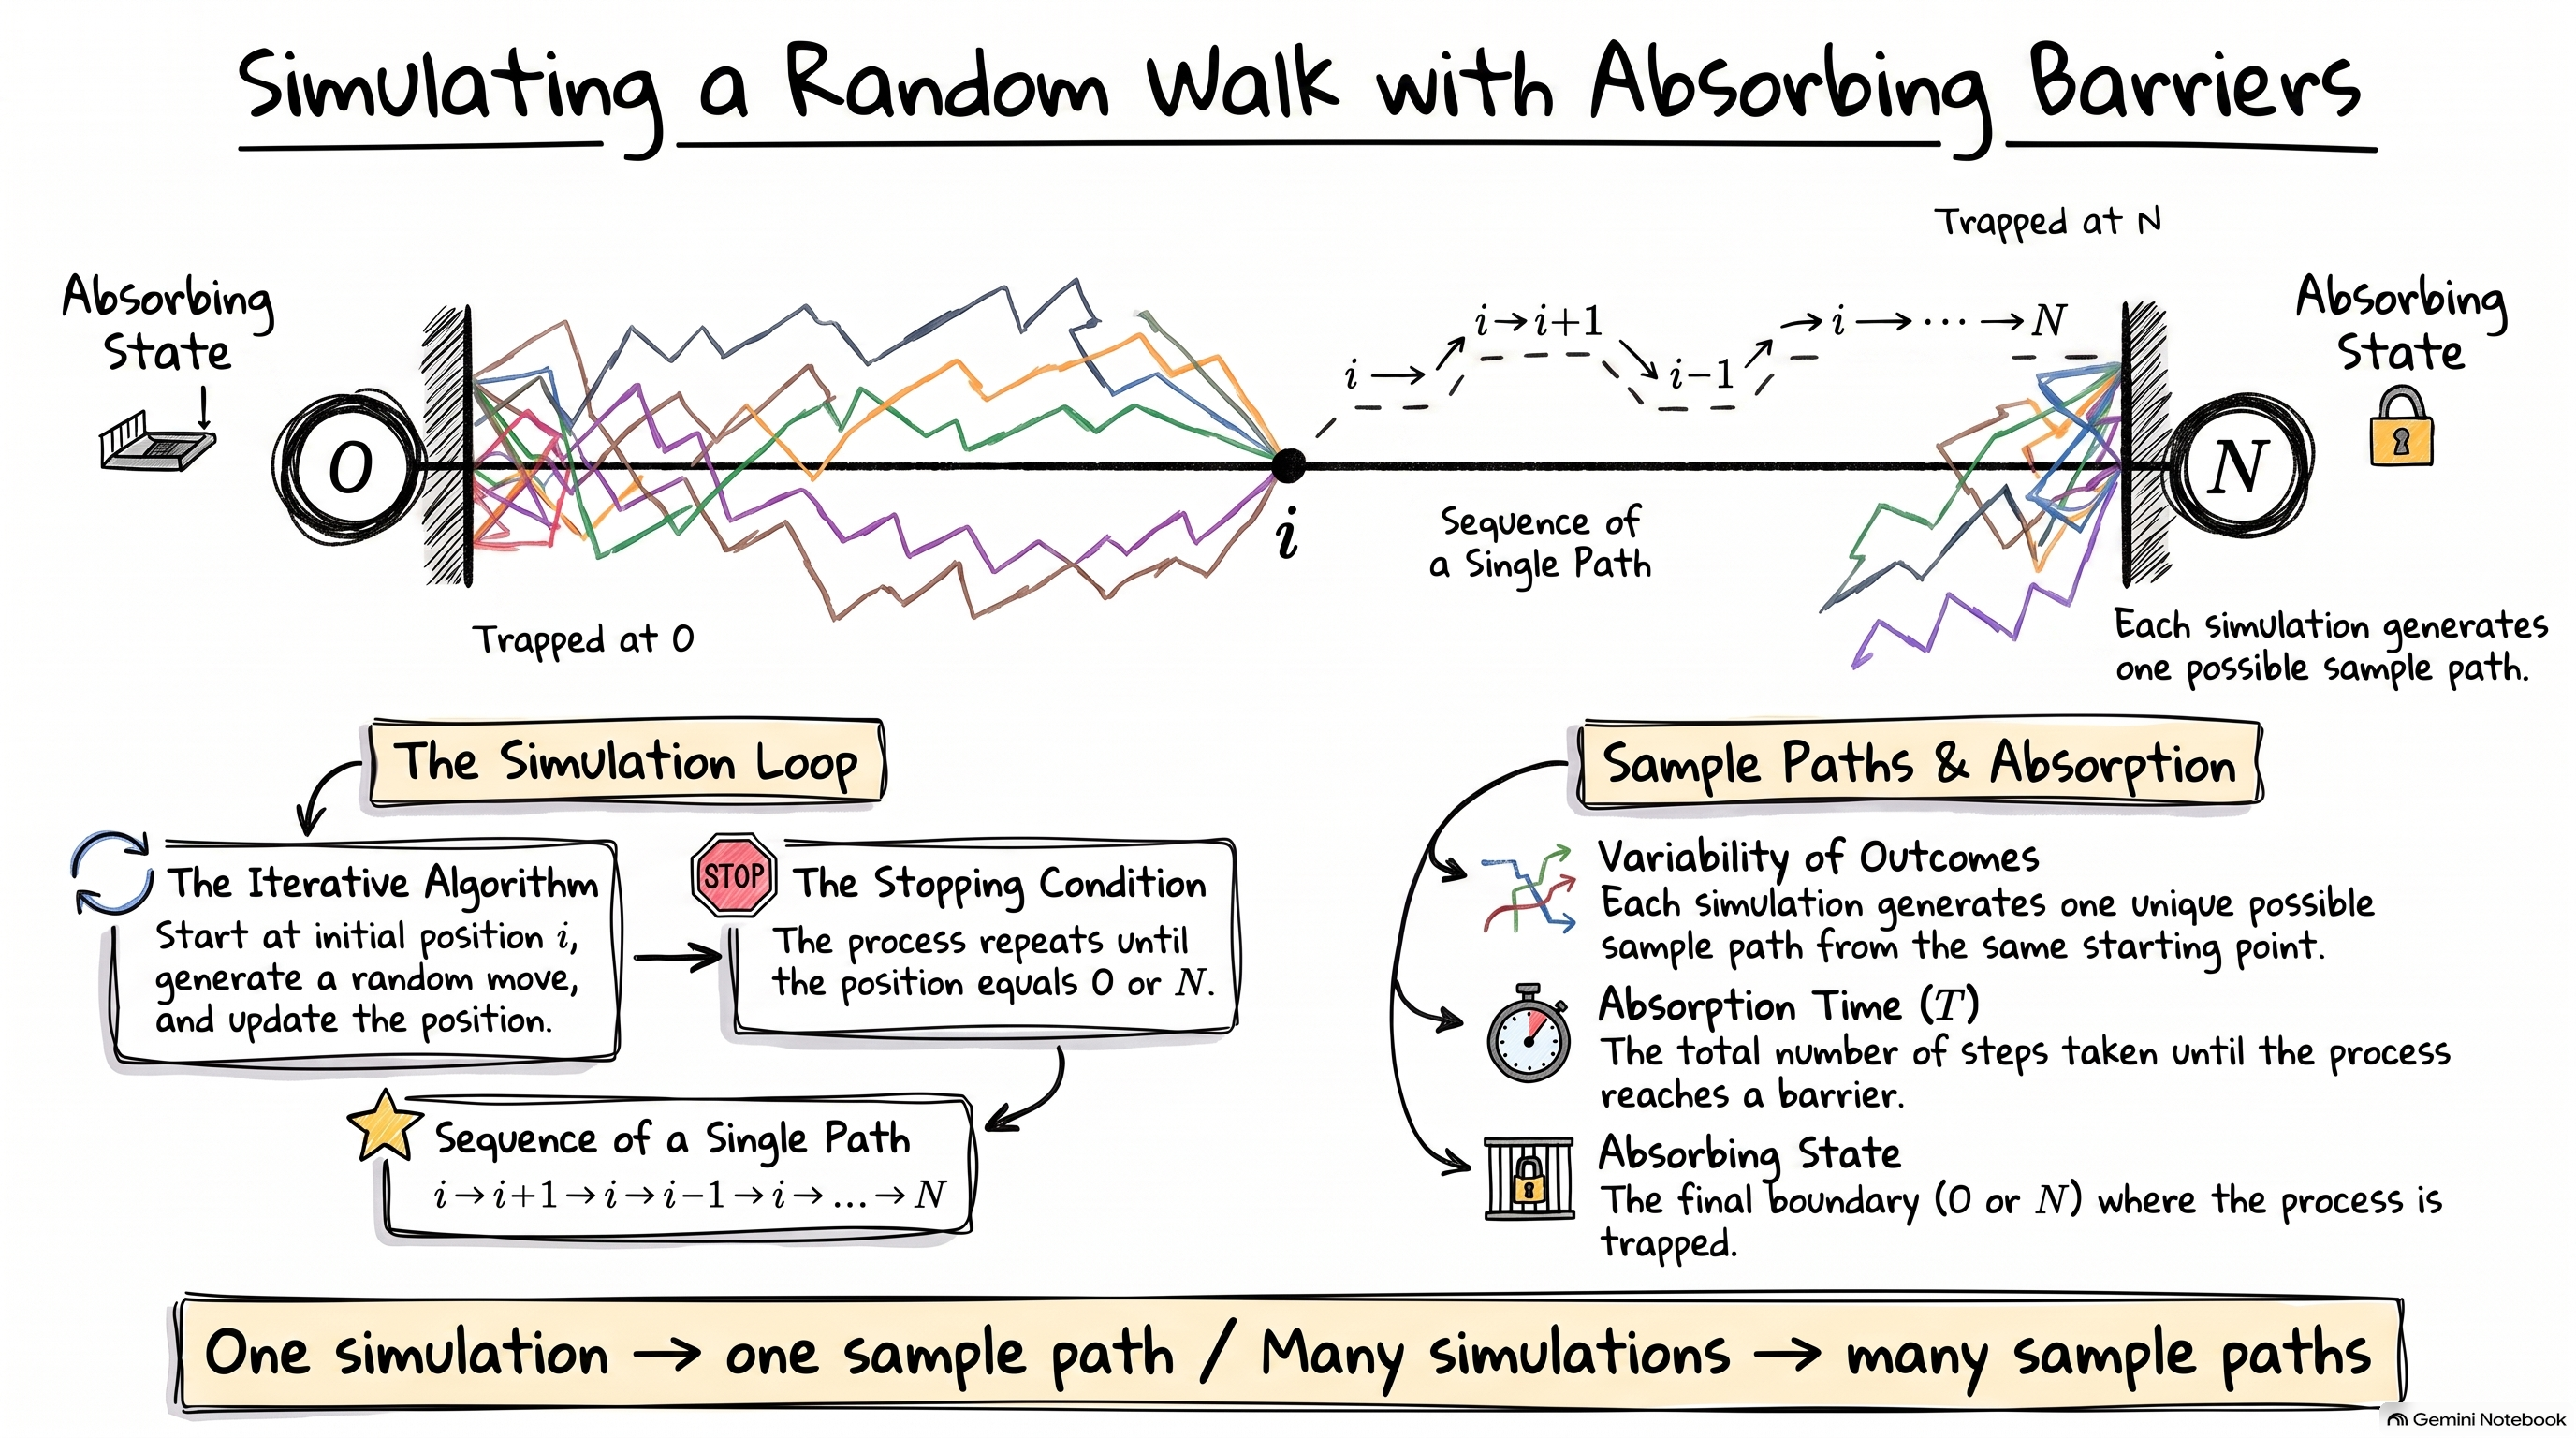
\includegraphics[width=0.8\linewidth,height=\textheight,keepaspectratio]{../figures/Random_Walk_Absorbing_Barrier_Simulation.png}

}

\caption{Random Walk Simulation}

\end{figure}%
\end{frame}

\begin{frame}{What can we learn from simulation?}
\protect\phantomsection\label{what-can-we-learn-from-simulation}
Each simulated path gives two quantities of interest:

\begin{itemize}
\tightlist
\item
  \textbf{Absorbing state:} whether the path ends at \(0\) or \(N\).
\item
  \textbf{Absorption time:} the number of transitions required to reach
  the absorbing state.
\end{itemize}

A collection of simulated paths can therefore be used to investigate

\[
\Pr(X_T=N\mid X_0=i)
\qquad\text{and}\qquad
\mathrm{E}[T\mid X_0=i].
\]

The simulation also shows the variability in the paths and in the time
taken to reach an absorbing state.
\end{frame}

\begin{frame}{Example: Simulating an absorbing random walk}
\protect\phantomsection\label{example-simulating-an-absorbing-random-walk}
Consider a fair random walk with absorbing barriers at \(0\) and \(10\),
starting from \(X_0=4\).

At each step, generate a move of \(+1\) or \(-1\), each with probability
\(1/2\). Stop the path when it reaches either \(0\) or \(10\).

A possible simulated path is

\[
4\rightarrow5\rightarrow4\rightarrow3\rightarrow4\rightarrow5
\rightarrow6\rightarrow7\rightarrow8\rightarrow9\rightarrow10.
\]

This path is absorbed at \(10\) after \(10\) steps.

The particular path and absorption time will vary each time the
simulation is performed.
\end{frame}

\begin{frame}{Example: Simulated sample paths}
\protect\phantomsection\label{example-simulated-sample-paths}
Several independent sample paths might produce the following results:

{\def\LTcaptype{none} % do not increment counter
\begin{longtable}[]{@{}rrrr@{}}
\toprule\noalign{}
Path & Starting state & Absorbing state & Time of absorption \\
\midrule\noalign{}
\endhead
1 & \(4\) & \(10\) & \(18\) \\
2 & \(4\) & \(0\) & \(8\) \\
3 & \(4\) & \(10\) & \(30\) \\
4 & \(4\) & \(0\) & \(12\) \\
5 & \(4\) & \(10\) & \(24\) \\
\bottomrule\noalign{}
\end{longtable}
}

Each row corresponds to one simulated sample path.

The \textbf{absorbing state} shows where the path ends, while the
\textbf{time of absorption} records how many transitions were required.
\end{frame}

\begin{frame}{Comparing simulation with theory}
\protect\phantomsection\label{comparing-simulation-with-theory}
For the fair random walk with \(N=10\) and \(X_0=4\), the exact
absorption probability at \(10\) is

\[
\Pr(X_T=10\mid X_0=4)=\frac4{10}=0.4.
\]

The exact expected time to absorption is
\(\mathrm{E}[T\mid X_0=4]=4(10-4)=24.\)

The five simulated paths above give three paths absorbed at \(10\), so
the simulated proportion is \(3/5=0.6\).

Their average absorption time is

\[
\frac{18+8+30+12+24}{5}=18.4.
\]

These simulated values are not expected to equal the theoretical values
exactly because only five paths were generated.
\end{frame}

\begin{frame}{More simulated paths}
\protect\phantomsection\label{more-simulated-paths}
Suppose we generate many independent sample paths.

The proportion of paths absorbed at \(10\) should become closer to the
exact probability \(0.4\) as the number of paths increases.

Similarly, the average absorption time should become closer to the exact
value \(24\).

This illustrates an important distinction:

\begin{itemize}
\tightlist
\item
  \textbf{Simulation} generates individual sample paths from the model.
\item
  \textbf{Monte Carlo estimation} uses many simulated paths to estimate
  quantities such as probabilities and expectations.
\end{itemize}
\end{frame}

\begin{frame}{Simulation as a computational tool}
\protect\phantomsection\label{simulation-as-a-computational-tool}
Simulation is particularly useful for visualising the behaviour of a
stochastic process.

For an absorbing random walk, it can show that

\begin{itemize}
\tightlist
\item
  different paths can have very different trajectories;
\item
  different paths can be absorbed at different boundaries;
\item
  the absorption time can vary substantially between paths;
\item
  starting closer to a boundary generally leads to faster absorption.
\end{itemize}

When exact calculations are available, simulation can be used to check
that the simulated results are consistent with the theoretical results.

When exact calculations are difficult or unavailable, simulation can
provide estimates of quantities of interest.
\end{frame}

\begin{frame}
\end{frame}

\section{Monte Carlo Methods}\label{monte-carlo-methods}

\begin{frame}{From simulation to estimation}
\protect\phantomsection\label{from-simulation-to-estimation}
Simulation generates individual sample paths. When many independent
paths are simulated, we can use the results to \textbf{estimate
quantities of interest}.

This approach is called a \textbf{Monte Carlo method}.

Consider a random walk with absorbing barriers at \(0\) and \(N\),
starting from \(X_0=i\). Suppose that \(M\) independent sample paths are
simulated.

For each path, record the absorption time \(T_m\) and whether the path
is absorbed at the upper barrier \(N\).
\end{frame}

\begin{frame}{Monte Carlo Estimation for Absorbing Random Walks}
\protect\phantomsection\label{monte-carlo-estimation-for-absorbing-random-walks}
\begin{figure}[H]

{\centering 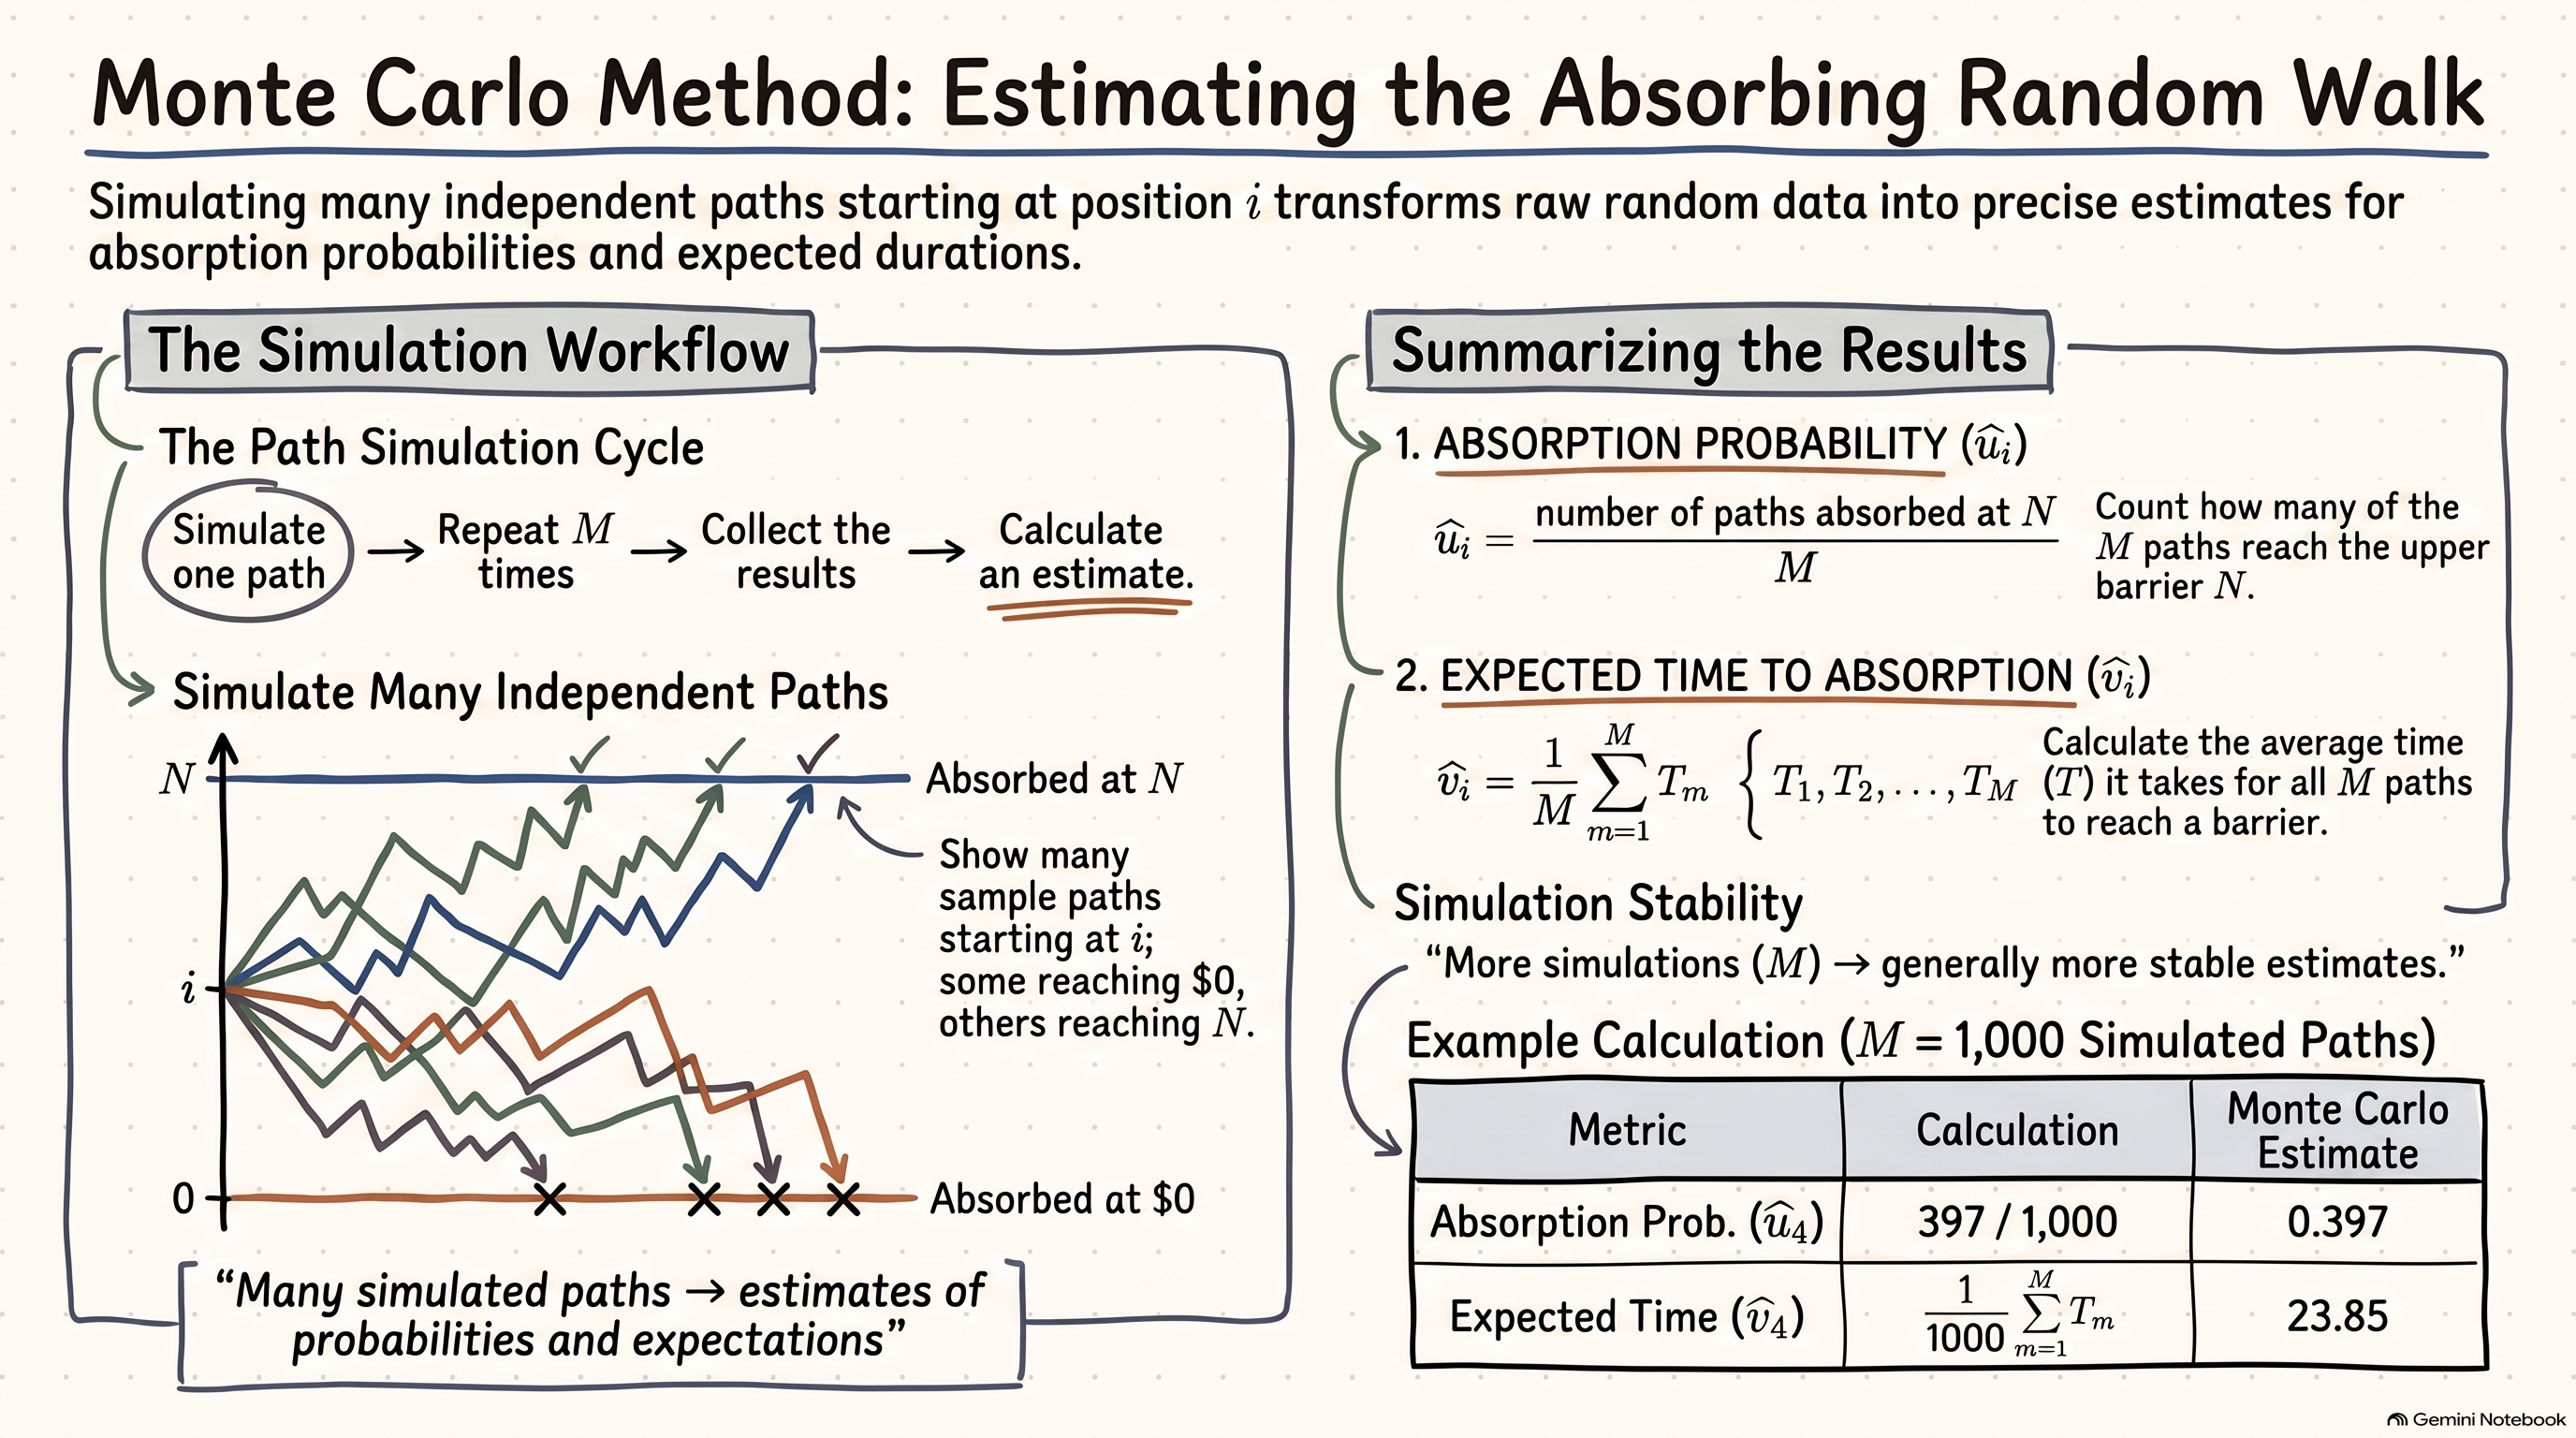
\includegraphics[width=0.75\linewidth,height=\textheight,keepaspectratio]{../figures/Monte_Carlo_Absorbing_Random_Walk.png}

}

\caption{Monte Carlo Estimation Results}

\end{figure}%
\end{frame}

\begin{frame}{Estimating an absorption probability}
\protect\phantomsection\label{estimating-an-absorption-probability}
Define the indicator

\[
I_m=
\begin{cases}
1, & \text{if path }m\text{ is absorbed at }N,\\
0, & \text{if path }m\text{ is absorbed at }0.
\end{cases}
\]

The proportion of paths absorbed at \(N\) is

\[
\widehat{u}_i=\frac{1}{M}\sum_{m=1}^{M}I_m.
\]

This provides a Monte Carlo estimate of

\[
u_i=\Pr(X_T=N\mid X_0=i).
\]

As \(M\) increases, \(\widehat{u}_i\) generally becomes closer to the
theoretical value \(u_i\).
\end{frame}

\begin{frame}{Estimating the expected time}
\protect\phantomsection\label{estimating-the-expected-time}
For the \(m\)th simulated path, let \(T_m\) be its absorption time.

The sample mean

\[
\widehat{v}_i=\frac{1}{M}\sum_{m=1}^{M}T_m
\]

provides a Monte Carlo estimate of

\[
v_i=\mathrm{E}[T\mid X_0=i].
\]

Thus, the same simulated paths can be used to estimate both

\[
\Pr(X_T=N\mid X_0=i)
\qquad\text{and}\qquad
\mathrm{E}[T\mid X_0=i].
\]
\end{frame}

\begin{frame}{Example: Monte Carlo estimation}
\protect\phantomsection\label{example-monte-carlo-estimation}
Consider a fair random walk with absorbing barriers at \(0\) and \(10\),
starting from \(X_0=4\).

Suppose \(M=1{,}000\) independent sample paths are simulated. Of these
paths, \(397\) are absorbed at \(10\).

The total of the \(1{,}000\) absorption times is \(23{,}850\).

Estimate the probability of absorption at \(10\) and the expected time
to absorption.
\end{frame}

\begin{frame}{Example: Monte Carlo estimation}
\protect\phantomsection\label{example-monte-carlo-estimation-1}
The estimated probability of absorption at \(10\) is

\[
\widehat{u}_4=\frac{397}{1{,}000}=0.397.
\]

The estimated expected time to absorption is

\[
\widehat{v}_4=\frac{23{,}850}{1{,}000}=23.85.
\]

Therefore,

\[
\boxed{\widehat{u}_4=0.397}
\qquad\text{and}\qquad
\boxed{\widehat{v}_4=23.85}.
\]
\end{frame}

\begin{frame}{Example: Comparing with exact results}
\protect\phantomsection\label{example-comparing-with-exact-results}
For a fair random walk with \(N=10\) and \(X_0=4\), the exact results
are

\[
u_4=\frac4{10}=0.4
\qquad\text{and}\qquad
v_4=4(10-4)=24.
\]

The Monte Carlo estimates are therefore close to the exact values:

{\def\LTcaptype{none} % do not increment counter
\begin{longtable}[]{@{}lrr@{}}
\toprule\noalign{}
Quantity & Exact value & Monte Carlo estimate \\
\midrule\noalign{}
\endhead
Absorption at \(10\) & \(0.400\) & \(0.397\) \\
Expected time & \(24.00\) & \(23.85\) \\
\bottomrule\noalign{}
\end{longtable}
}

The estimates will vary from one simulation to another because they are
based on a finite number of simulated paths.
\end{frame}

\begin{frame}{Simulation error}
\protect\phantomsection\label{simulation-error}
A Monte Carlo estimate is based on a finite number of simulated paths
and is therefore subject to \textbf{simulation error}.

Increasing \(M\) generally makes the estimates more stable and closer to
the theoretical values.

However, increasing \(M\) does not guarantee that an estimate is exactly
equal to the theoretical value.

The aim is to obtain an estimate with sufficiently small simulation
error for the application.
\end{frame}

\begin{frame}{Why use Monte Carlo methods?}
\protect\phantomsection\label{why-use-monte-carlo-methods}
For the absorbing random walk, we can derive exact formulas such as

\[
u_i=\frac{i}{N}
\qquad\text{and}\qquad
v_i=i(N-i)
\]

for the fair case.

For more complicated Markov chains, however, exact calculations may
require large systems of equations or may not have a simple analytical
solution.

Monte Carlo methods then provide a practical way to estimate quantities
of interest by simulating the process repeatedly.
\end{frame}

\begin{frame}{Key idea}
\protect\phantomsection\label{key-idea-2}
The three approaches play different roles:

\begin{itemize}
\tightlist
\item
  \textbf{Analytical calculation:} derives exact probabilities or
  expectations when possible.
\item
  \textbf{Simulation:} generates individual sample paths to study the
  behaviour of the process.
\item
  \textbf{Monte Carlo estimation:} uses many simulated paths to estimate
  probabilities, expectations, and other quantities of interest.
\end{itemize}

Monte Carlo methods therefore extend the use of simulation from
\textbf{observing the process} to \textbf{estimating its properties}.
\end{frame}




\end{document}
